
\chapter{Classical numerical results and Benchmarks} % Main chapter title

\label{Chapter3} % Change X to a consecutive number; for referencing this chapter elsewhere, use \ref{ChapterX}

By last section we saw the American put was an example of an option that required numerical procedures to be priced fair. The American put is far from the only example of a derivative with not a closed form solution. The two first sections deals with pricing American put option with 1 underlying stock, where in the last section we try to price options with several underlying risky assets. \\

The two first sections is two classical valuing algorithms in computational finance the Binomial model \parencite{CRR} and the Least Square Monte Carlo (LSM \parencite{lsm}) approach with one underlying asset. The binomial model is an example of a strategy to approximate the B-S model and the LSM is a method trying to solve the variational inequalities. We could also have chosen to solve the free boundary problem with implicit finite difference, but we chose to focus on the two other numerical procedures. The final section in this chapter will be trying to value exotic options with several underlying assets. Here we will extend the binomial pricing model to multidimensional (\parencite{NEK} and \parencite{BEG}) and provide some closed form solutions (\parencite{Johnson87} and \parencite{Ouwehand2006}). Hence the chapter have two purposes to gain insight into valuation for exotic options and provide some benchmarks for the Neural Network in the coming chapters.

%----------------------------------------------------------------------------------------
%	SECTION 1
%----------------------------------------------------------------------------------------
\section{Binomial Pricing model}
The classical \parencite{CRR} presented in this section will be used for pricing an American put stock option and to build the foundation for the multidimensional binomial model \parencite{BEG}.
The Binomial model provides an intuitive and easy implementable model for valuing American and European options. The Binomial model comes handy, when no analytical model exists e.g. an American put option. The Binomial model also has its limitations, because it is not suited for valuing path dependent options or options with a lot of several underlying factors. The key difference on the Binomial model and the other numerical procedures is that the Binomial model is build on a discrete framework. \\

The central concepts arbitrage and completeness from continuous time also work in the discrete time setup. The paper \parencite{CRR} which introduced the binomial model to option pricing came after the Black-Scholes model described in section \ref{Chapter2} \parencite{B-S-Paper}. The main reason for developing a model in discrete time, is that the the discrete time approach gives a simplified model in terms of the mathematics and highlights the essential concepts in arbitrage theory. You can argue that the simpler mathematics in this model makes the binomial model more instructive and clear. Besides being easier to understand for non-mathematician it works nicely with other options than the European options like American options.\\

Even though we assume the stock price moves at discrete time instead in continuous time. It can actually be shown for a European Option that if the number of time-steps in the tree approaches infinity, then the Binomial model will converge to the continuous time closed form solution for a European option \parencite{CRR} \parencite{Hull}. Hence the binomial pricing model will be equivalent with the continuous time analytical pricing model derived by Fischer Black and Myron Scholes in the limit for European options \parencite{CRR}.\\

To value a American put option, we lay out all the possible path of the stock, based on the $S_0,\sigma$ and $T$. We need to specify the number of time-steps ($\Delta t = \frac{T}{N} \ where \ N=No. \ of  \ steps$) for the tree, where for each step, we add another possible value for the stock. We only add 1 more possibility for each time-step because the tree recombines. The precision for the algorithm increases with the number of steps and the option value stabilizes (see Figure \ref{fig:binConv}). For valuing an American put option, we value the exercise value at maturity (time T) for all possible outcomes for the stock. Then we use backward induction where we compare the intrinsic value with the conditional expectation, where we choose the maximum of these two \parencite{Hull}. 
 
\begin{figure}[th]
\centering
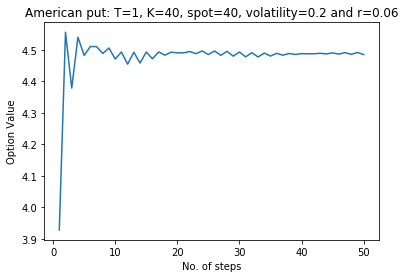
\includegraphics{Figures/binConv.png}
\decoRule
\caption[Convergence of Binomial model]{}
\label{fig:binConv}
\end{figure}

%-----------------------------------
%	SUBSECTION 1
%-----------------------------------

\subsection{Mathematics in Binomial valuation model}
The mathematics behind the Binomial model is simple and we will in this section provide the basic mathematics. First we need to construct the tree, then afterwards work backwards in the tree for valuation. For each time step ($\Delta t$), we assume the stock (S) can move up (u) or down (d). In order to avoid arbitrage we find the risk neutral measure q (martingale measure) for the binomial tree, where q is the probability for the stock moves up. The risk neutral measure q is chosen s.t. the expected return is the risk-free rate r.

\begin{theorem}\label{RNVF-Discrete}
\textbf{Risk-neutral valuation formula in discrete time. }
Assume there exists a risk free asset. Then the market is arbitrage free if and only if there exists a risk neutral measure $Q \sim P$ s.t.
\begin{align}
s= \exp(- r \Delta t) \cdot E^Q[S(t+\Delta t)|S(t)=s] 
\end{align}
Where $\Delta t$ is a single time-step.
\end{theorem}
From the above theorem, we can calculate the risk neutral measure as:\\
$$q=\frac{e^{\Delta t}-d}{u-d}$$

The d and u is chosen s.t. they match volatility. So we choose:
$$u= \exp(\sigma \sqrt{\Delta t}) \quad d= \exp(-\sigma \sqrt{\Delta t})$$
Now we have determined the three parameters needed for constructing a binomial tree \parencite{CRR} \parencite{Hull} \parencite{finKont}.\\

We want to value an American put option, hence we need to work backward in the tree and comparing in each node the intrinsic value with the conditional expectation (see theorem \ref{RNVF-Discrete}) by:
\begin{equation}
max\{ K-S(t), \exp(- r \Delta t) \cdot E^Q[P(t+\Delta t,T)|P(t,T)=p] \}
\end{equation}
The comparison will be applied for every node in each time-step $\Delta t$  and all the way back in time to the initialization date. By this procedure we get present value of the American option at initialization.

%----------------------------------------------------------------------------------------
%	SECTION 2
%----------------------------------------------------------------------------------------

\section{Least Square Monte Carlo Method}
The other classical result in this section is of an different nature, because it is based on simulation and linear regression. In our setting we regress the expected payoff by continuation of the contract and compare it to the intrinsic value. The dependent variable in the regression is the expected value of continuation and the independent variables is a set of orthogonal basis functions in $L^2(\Omega, \mathcal{F}, Q)$ of the simulated paths. Typical choices for basis functions could be weighted Laguerre -, Hermit -, and Jacob polynomials. This kind of regression is a nonlinear expansion of the linear model. In order to create data, we will simulate paths according to the underlying risky asset. 

%-----------------------------------
%	SUBSECTION 1
%-----------------------------------
\subsection{LSM method for an American put}           
We want to valuate an American put option with a stock as underlying asset. We take the same assumptions as in Chapter \ref{Chapter2} (see assumption \ref{BS-Assumption}) except the option is an American option. Hence in order to simulate the paths of the stock, we simulate from an GBM: $dS(t)=rSdt + \sigma S dW_t$ where $\sigma$ and r is constant (see solution to SDE equation \ref{GBM}). We simulate 100.000 paths for the stock. Like in the binomial model, we work backward to decide the optimal stopping time. The computer is discrete, hence we simulate the stock path as an Bermuda option, where we have 50 time-steps per year. I.e. we approximate the American option with a Bermudan option on same underlying. \\

At maturity the cash flow from the option is the same as for an European put option, hence the cash flow from each path is $C(\omega,T;T, T)=max(K-S_T,0)$. We use the notation $C(\omega, s; t, T)$ denote the path of cash flows generated by the option condition on the option not being exercised before t and the option holder follow the optimal stopping strategy for all s, $t<s\leq T$.
(inspired by \parencite{lsm} p. 121). The continuation value is given by:
\begin{equation}\label{continuation-value}
\begin{split}
F(\omega; t_k)=E^Q[\sum_{j=k+1}^K \exp(-\int_{t_k}^{t_j} r(\omega,s) ds)C(\omega,t_j; t_k, T)|\mathcal{F}_{t_k}]
\end{split}
\end{equation}
where $r(\omega,t)$ is risk free interest rate, and the $\mathcal{F}_{t_k}$ is the filtration at time $t_k$.\\

The optimal stopping strategy is then by comparing this continuation value with the intrinsic value at each time step. By working backward in time until the initialization of the option, we have specified the optimal stopping times and the cash flows associated with exercising at the optimal stopping times. To estimate the condition expectation in equation \ref{continuation-value}, we regres with the basis functions taking on the underlying asset for the option being the independent variable:
$$F(\omega;t_{K-1})= \sum_{j=0}^\infty a_j L_j(X)$$
where a is the coefficients for the regression, L is the basis function, where the argument is the underlying asset $X$ \parencite{lsm}.

%-----------------------------------
%	SUBSECTION 2
%-----------------------------------

\subsection{Numerical results}
By the above two algorithms for valuation, we choose to vary spot, volatility and maturity for pricing an American put option with K=40 and r=0.06. This table will serve as reference for the machine learning algorithm in chapter (!TODO chapter for machine learning). For the binomial tree we use 100 time-steps, which gives stable results (compare to figure \ref{fig:binConv}) and for the LSM we use $10^5$ paths with 50 time-steps per year. The European option is valued by using BS closed form solution for a call option (see proposition \ref{BS-price-EuroCall}) and Put-call parity (see proposition \ref{Put-call-parity}).
\begin{table}[th]
\caption{Valuation of American put option with K=40 and r=0.06.}
\label{tab:treatments}
\centering
\begin{tabular}{l l l l l l l }
\toprule
\textbf{Spot} & \textbf{$\sigma$} & \textbf{T} & \textbf{Closed form European} & \textbf{Binomial Tree} & \textbf{LSM} & \textbf{abs. diff.} \\
\midrule
36 & 0.2 & 1 & 3.844 & 4.488 & 4.478 & 0.010\\
36 & 0.2 & 2 & 3.763 & 4.846 & 4.828 & 0.018\\
36 & 0.4 & 1 & 6.711 & 7.119 & 7.092 & 0.027\\
36 & 0.4 & 2 & 7.700 & 8.508 & 8.500 & 0.008\\
38 & 0.2 & 1 & 2.852 & 3.260 & 3.245 & 0.015\\
38 & 0.2 & 2 & 2.991 & 3.748 & 3.735 & 0.013\\
38 & 0.4 & 1 & 5.834 & 6.165 & 6.144 & 0.021\\
38 & 0.4 & 2 & 6.979 & 7.689 & 7.665 & 0.024\\
40 & 0.2 & 1 & 2.066 & 2.316 & 2.313 & 0.003\\
40 & 0.2 & 2 & 2.356 & 2.885 & 2.881 & 0.004\\
40 & 0.4 & 1 & 5.060 & 5.310 & 5.326 & 0.016\\
40 & 0.4 & 2 & 6.326 & 6.914 & 6.908 & 0.006\\
42 & 0.2 & 1 & 1.465 & 1.622 & 1.622 & 0.000\\
42 & 0.2 & 2 & 1.841 & 2.217 & 2.212 & 0.005\\
42 & 0.4 & 1 & 4.379 & 4.602 & 4.596 & 0.006\\
42 & 0.4 & 2 & 5.736 & 6.264 & 6.243 & 0.021\\
44 & 0.2 & 1 & 1.017 & 1.117 & 1.113 & 0.004\\
44 & 0.2 & 2 & 1.429 & 1.697 & 1.688 & 0.009\\
44 & 0.4 & 1 & 3.783 & 3.956 & 3.962 & 0.006\\
44 & 0.4 & 2 & 5.202 & 5.656 & 5.649 & 0.007\\
\bottomrule\\
\end{tabular}
\end{table}
We see the maximum difference between the two algorithms is 0.027 at S=38, $\sigma=0.4$ and T=2. The other obvious fact is that the European put has a lower value than its American counterpart, because the continuous exercise feature adds additional value to the put option. 


%----------------------------------------------------------------------------------------
%	SECTION 3
%----------------------------------------------------------------------------------------

\section{Benchmarks in higher dimensions}\label{BMHiggerDim}
In this section will we provide closed form solution for some special cases of European multivariate contingent claims. Furthermore we present a lattice approach in multidimensional for pricing both European and American multivariate contingent claims. The basic assumptions and results are given in section \ref{MultiDimModel}.

\subsection{Analytical formulas for Rainbow options}
We derive closed form solutions to European call and put options depending on several variables, for simplicity will we focus on pricing options with 2 or 3 underlying stocks. We apply the intuition given in \parencite{Johnson87} and the results given in \parencite{Ouwehand2006}. The options we will consider is the geometric mean -, maximum - and minimum call option.

\subsubsection{Geometric basket call option}
For a geometric basket call option the contract function is given by:
\begin{align*}
\Phi(S(T))=\max\{ (\prod_{i=1}^{n} S_i(T))^{\frac{1}{n}}-K,0 \}
\end{align*}
The key to derive closed form solution is the known result that the sum of normal random variables are multivariate normal distributed.
This implies that the product of lognormal random variables are multivariate log-normal distributed. Since: 
\begin{equation*}
\begin{split}
\exp(x+y)=\exp(x)\cdot \exp(y) \\
X \sim \mathcal{N}(\mu,\sigma^2) \Rightarrow Y = \exp(X)\sim LN(\mu, \sigma^2)
\end{split}
\end{equation*}

We assume as in section \ref{MultiDimModel} that the stocks price process follows a GBM, hence:
\begin{equation}
\begin{split}
(\prod_{i=1}^{n} S_i(T))^{\frac{1}{n}} = (\prod_{i=1}^{n} S_i(0))^{\frac{1}{n}} \exp((r-\frac{1}{2n}\sum_{i=1}^{n}\sigma_i^2)T + \frac{1}{n} \sum_{i=1}^{n} \sigma_i W_i(T))
\end{split}
\end{equation}
By defining
\begin{align}
\sigma = \frac{1}{n} \sqrt{\sum_{i=1}^{n} \sigma_i^2 + 2 \sum_{i\neq j} \rho_{i,j}\sigma_i \sigma_j}\\
F=(\prod_{i=1}^{n} S_i(0))^{\frac{1}{n}} \exp((r-\frac{1}{2n}\sum_{i=1}^{n}\sigma_i^2)T + \frac{1}{2} \sigma^2 \cdot T
\end{align}
We arrive at the price by skipping some arguments:
\begin{equation}
\Pi(t,\mathcal{X})=\exp(-r*(T-t))\bigg(F N(d_1) - K N(d_2) \bigg)
\end{equation}
where $d_1=\frac{\ln(\frac{F}{K}) + \frac{1}{2} \sigma^2 T}{\sigma \cdot \sqrt{T}}$ and $d_2=d_1-\sigma \sqrt{T}$

\subsubsection{Options on the Maximum or the Minimum of Several Assets}
Here we restrict ourselves to consider the case with three underlying stocks like in \parencite{BEG} and \parencite{Ouwehand2006}, but the formula can be generalized to higher dimensions. The contract function we will consider is:
\begin{enumerate}
\item[•] Best of assets or cash: $\Phi(S(T))=\max\{S_1,S_2,\ldots,S_n,K\}$
\item[•] Call on max: $\Phi(S(T))=\max\{\max(S_1,S_2,\ldots,S_n)-K,0\}$
\end{enumerate}
We use n=3 because it shows the generality without the notation becomes to cumbersome.

We use the martingale framework developed in section \ref{MultiDimModel} to value these exotic options. The key is to choose the numeraire to a risky assets instead of the bank account. By results from section \ref{MultiDimModel} the processes are still Q-martingales given the numeraire is strictly postive. So under the asssumption the arbitrage free and complete market it follows:
$$S_0(t)E^{Q_0}_t[\frac{X_T}{S_0(T)}]=S_1(t)E^{Q_1}_t[\frac{X_T}{S_1(T)}]$$

\paragraph{Best of assets or cash}
The best of assets will both provide a price and the method for pricing call on max and min. We assume WLOG n=4 and define the payoff as for the i'th asset:
$$S_i(T) \cdot 1_{S_i(T)>S_j(T): i\neq j}$$
Hence the best of assets derivative is a sum of above equation for each asset. So we are considering four cases, because we assumed WLOG n=4. \\

For i=1 we set $S_1$ to be the numeraire asset with martingale measure $\mathbb{Q}_1$. then we see by using RNVF (see proposition \ref{RNVF}):
\begin{equation}
\begin{split}
\Pi_1(t, \mathcal{X})&=S_1(t)E_t^{Q_1}[1_{S_1(T)>S_2(T), S_1(T)>S_3(T), S_1(T)>S_4(T)}]\\
&=S_1(t) Q_1[\ln(\frac{S_2(T)}{S_1(T)})<0, \ln(\frac{S_3(T)}{S_1(T)})<0, \ln(\frac{S_4(T)}{S_1(T)})<0]
\end{split}
\end{equation}
By cycling through the numeraires we get four derivatives that we need to add together for optaining the fair price for best of assets $\Pi_{max}(t,\mathcal{X})$. Before we can proceed we need to find the probaility under the $Q$-martingale measure. By using Ito's lemma (see \ref{Ito}):
\begin{align*}
\ln(\frac{S_i(T)}{S_j(T)})\sim \mathcal{N}(\ln(\frac{S_i(T)}{S_j(T)}) - \frac{1}{2}\sigma_{i/j}^2 \cdot (T-t), \sigma_{i/j}\sqrt{T-t})
\end{align*}
where $\sigma_{i/j}^2=\sigma_i^2+\sigma_j^2-2\rho_{ij}\sigma_i \sigma_j$.\\

Besides using the definition for $d_1$ and $d_2$ in proposition \ref{BS-price-EuroCall} we define:
\begin{align}
d^{i/j}_1 =\frac{1}{\sigma\cdot \sqrt{T-t}} \cdot \bigg( \ln(\frac{S_i}{S_j}) + \frac{1}{2} \sigma_{i/j}^2 \cdot (T-t) \bigg)\\
d^{i/j}_2=d^{i/j}_1-\sigma_{i/j} \sqrt{T-t}
\end{align}
Furthermore the correlation between $\ln(\frac{S_i(T)}{S_j(T)})$ and $\ln(\frac{S_i(T)}{S_j(T)})$ is given by (see page 5 \parencite{Ouwehand2006}):
\begin{align}
\rho_{ij,k}= \frac{\rho_{ij}\sigma_i \sigma_j - \rho_{ik}\sigma_i \sigma_k - \rho_{kj}\sigma_k \sigma_j + \sigma_k^2}{\sqrt{(\sigma_i^2 + \sigma_k^2 - 2\rho_{ik}\sigma_i \sigma_k)\cdot(\sigma_j^2 + \sigma_k^2 - 2\rho_{jk}\sigma_j \sigma_k)}}
\end{align}
Hence:
$$Q_1[\ln(\frac{S_2(T)}{S_1(T)})<0, \ln(\frac{S_3(T)}{S_1(T)})<0, \ln(\frac{S_4(T)}{S_1(T)})<0]=N_3(-d_2^{2/1},-d_2^{3/1},-d_2^{4/1}, \rho_{23,1}, \rho_{24,1}, \rho_{34,1})$$
Cycling through each derivative, we get:
\begin{equation}\label{BestAsset}
\begin{split}
\Pi_{max}(t,\mathcal{X})&=S_1(t) N_3(-d_2^{2/1},-d_2^{3/1},-d_2^{4/1}, \rho_{23,1}, \rho_{24,1}, \rho_{34,1}) \\
&+S_2(t) N_3(-d_2^{1/2},-d_2^{3/2},-d_2^{4/2}, \rho_{13,2}, \rho_{14,2}, \rho_{34,2})\\
&+S_3(t) N_3(-d_2^{1/3},-d_2^{2/3},-d_2^{4/3}, \rho_{12,3}, \rho_{14,3}, \rho_{24,3}) \\
&+S_4(t) N_3(-d_2^{1/4},-d_2^{2/4},-d_2^{3/5}, \rho_{12,4}, \rho_{13,4}, \rho_{23,4})
\end{split}
\end{equation}
We can extend the above result to best of assets and cash by letting $S_4(t)=K\exp(-r(T-t))$, where K do not have any volatilty and also independent of the other assets, hence \eqref{BestAsset} becomes:
\begin{equation}\label{BestAssetOrCash}
\begin{split}
\Pi_{max}(t,\mathcal{X})&=S_1(t) N_3(-d_2^{2/1},-d_2^{3/1},d_1^{1}, \rho_{23,1}, \rho_{24,1}, \rho_{34,1}) \\
&+S_2(t) N_3(-d_2^{1/2},-d_2^{3/2},d_1^{2}, \rho_{13,2}, \rho_{14,2}, \rho_{34,2})\\
&+S_3(t) N_3(-d_2^{1/3},-d_2^{2/3},d_1^{3}, \rho_{12,3}, \rho_{14,3}, \rho_{24,3}) \\
&+K\cdot \exp(-r(T-t)) N_3(-d_2^1,-d_2^2,-d_2^3, \rho_{12}, \rho_{13}, \rho_{23})
\end{split}
\end{equation}

\paragraph{Call on max and call on min}
From \eqref{BestAssetOrCash} is easy to see the call max fair price is:
\begin{equation}\label{callMax}
\begin{split}
\Pi_{cmax}(t,\mathcal{X})&=S_1(t) N_3(-d_2^{2/1},-d_2^{3/1},d_1^{1}, \rho_{23,1}, \rho_{24,1}, \rho_{34,1}) \\
&+S_2(t) N_3(-d_2^{1/2},-d_2^{3/2},d_1^{2}, \rho_{13,2}, \rho_{14,2}, \rho_{34,2})\\
&+S_3(t) N_3(-d_2^{1/3},-d_2^{2/3},d_1^{3}, \rho_{12,3}, \rho_{14,3}, \rho_{24,3}) \\
&-K \exp(-r(T-t)) \cdot\bigg(1 - N_3(-d_2^1,-d_2^2,-d_2^3, \rho_{12}, \rho_{13}, \rho_{23})\bigg)
\end{split}
\end{equation}

To derive put max we can utilize a put-call-parity (see page 6 \parencite{Ouwehand2006}), but it takes a different form than the one presented in \ref{Chapter2} (see \ref{put-call-parity}). The relationship for the exotic call options:
$$V_c(K)+K\exp(-r\cdot (T-t)) = V_p(K)+V_c(0)$$
Where $V_c(K)$ is the value of the exotic call option.

These options will serve as benchmark for the multivariate lattice approach, and for pricing the call on min see \parencite{Ouwehand2006}.


\subsection{Lattice approach for multivariate contingent claims}
